%!TEX root = ../book.tex
\chapter{Path Planning}\label{chap:pathplanning}

Path planning is an important primitive for both autonomous mobile robots and manipulators; it allows a robot to find a path between two points.
A \textsl{path}\index{Path} is formally defined as a set of poses from a starting configuration to an ending configuration that respect a set of specifications (for example, avoiding obstacles for a mobile base or respecting a specific force profile at the end effector of a manipulator). It differs from the concept of \textsl{trajectory}\index{Trajectory} in that a trajectory is the execution (i.e., parametrization) of a path over time.
Depending on the choice of the planning algorithm, a path could satisfy various degrees of optimality with respect to some criteria such as minimizing path length, minimizing turns, or minimizing the amount of braking.
Algorithms to find a shortest path are important not only for robotics applications, but also in network routing, video games, and understanding protein folding.

Path planning requires a suitable representation of the environment (e.g., the map introduced in \cref{chap:mapping}) and a perceptual understanding of the robot's location with respect to such representation---which will be treated in \cref{chap:localization}. We will assume for now that the robot is able to localize itself, is equipped with a map, and is capable of avoiding temporary obstacles on its way. The goals of this chapter are to:

\begin{itemize}
\item understand the difference between graph-based and sampling-based planning algorithms,
\item explain basic path planning algorithms ranging from Dijkstra, to A*, D* and RRT,
\item introduce variations of the path planning problem, such as coverage path planning.
\end{itemize}

\section{Graph-based planning algorithms}

The problem to find a ``shortest'' path from one vertex to another through a connected graph is of interest for multiple domains, most prominently network routing for the internet, where it is used to find an optimal route for a data packet.
The term ``shortest'' here is defined as the minimum cumulative edge cost, which could be physical distance (in a robotic application), delay (in a networking application), or any other metric that is relevant for the task. An example graph with arbitrary edge lengths is shown in \cref{fig:pathproblem}.

\begin{figure}[!htb]
    \centering
    % 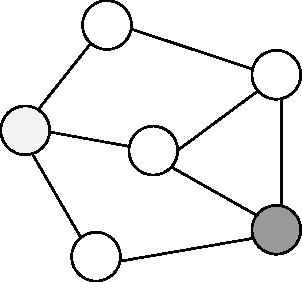
\includegraphics[width=0.6\textwidth]{figs/pathproblem}
    \def\svgwidth{0.6\textwidth}
    \import{./figs/}{pathproblem.pdf_tex}
    \caption{A generic path planning problem from vertex I to vertex VI. The shortest path is I-II-III-V-VI, and has length of $13$. \label{fig:pathproblem}}
\end{figure}

\subsection{Considerations about the robot embodiment}

In the vast majority of path planning algorithms, the robot is treated as a point-mass element with no volume. In order for a path to be executed on the robot, it is important to take into account the physical embodiment of the robot and its non-zero volumetric occupancy, which complicates the path planning process.
It is possible for the robot to be reduced to a point-mass while growing all obstacles by the length of the longest extension of the robot from its center (for a circular robot, its radius). This representation is known as \textsl{configuration space}\index{Configuration space} as it reduces the representation of the robot to its controllable degrees of freedom (e.g., its $x$ and $y$ coordinates in the plane for a robot capable of planar translation). An example is shown in \cref{fig:cspace}. The configuration space can now either be used as a basis for a grid map or a continuous representation.

\begin{figure}[!htb]
    \centering
    % 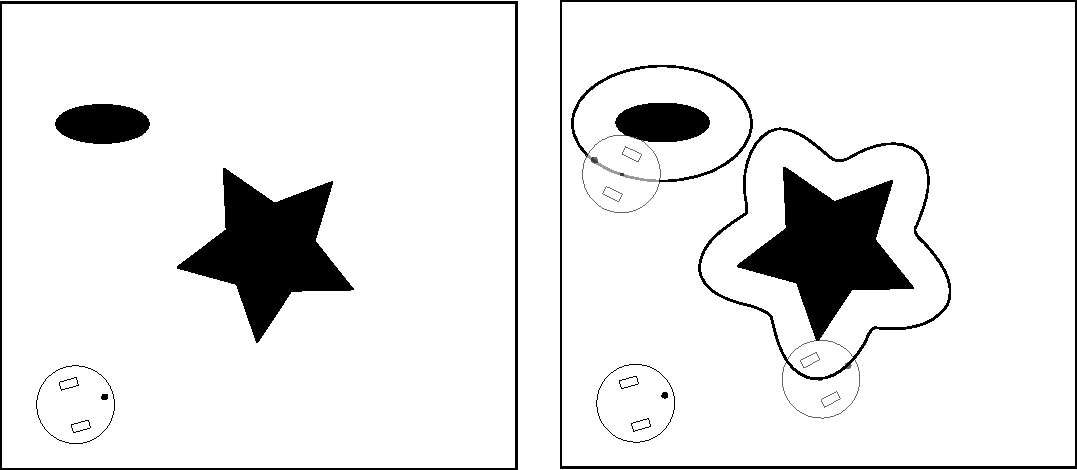
\includegraphics[width=0.9\textwidth]{figs/configurationspace}
    \def\svgwidth{0.9\textwidth}
    \import{./figs/}{configurationspace.pdf_tex}
    \caption{A map with obstacles and its representation in configuration space, which can be obtained by growing each obstacle by the robot's extension. \label{fig:cspace}}
\end{figure}

\subsection{Dijkstra's algorithm}\index{Dijkstra's Shortest Path Algorithm}
\screencast{https://youtu.be/_lHSawdgXpI}{dijkstra}

One of the earliest and simplest algorithms for path planning is Dijkstra's algorithm \cite{dijkstra1959note}. Given a map, Dijkstra is an iterative process where, starting from the initial starting configuration, the algorithm marks all its direct neighbors with the (possibly unitary) cost to reach them. It then proceeds to inspect the neighboring vertex with the lowest cost and all its adjacent vertices and marks them with the cost to get to them via the vertex under consideration. Once all neighbors of a vertex have been checked, the algorithm proceeds to the vertex with the next lowest cost. Once the algorithm reaches the goal vertex, it terminates and the robot can follow the edges pointing towards the lowest edge cost.

In the example in \cref{fig:pathproblem}, Dijkstra would first mark nodes II, III and IV with cost $3$, $5$ and $7$ respectively. It would then continue to explore all edges of node II, which so far has the lowest cost. This would lead to the discovery that node III can actually be reached in $3+1<5$ steps, and node III would therefore be relabeled with cost $4$. In order to completely evaluate node II, Dijkstra needs to evaluate the remaining edges before moving on and label node VI with $3+12=15$.
%
The node with the lowest cost is now node III (cost of $4$). We can now relabel node VI with $14$, which is smaller than 15, and label node V with $4+5=9$, whereas node IV remains at $4+3=7$. Although we have already found two paths to the goal, one of which better than the other, we cannot stop as there still exist nodes with unexplored edges and overall cost lower than $14$. Indeed, continuing to explore from node V leads to a shortest path I-II-III-V-VI of cost $13$, with no remaining nodes to explore.

As Dijkstra would not stop until there is no node with lower cost than the current cost to the goal, we can be sure that a shortest path will be found if it exists. We can therefore say that Dijkstra is both \textsl{complete} and optimal.\index{Complete (algorithm)}

As Dijkstra will always explore nodes with the least overall cost first, the environment is explored comparably to a wave front originating from the start vertex, eventually arriving at the goal. This is of course highly inefficient, in particular if Dijkstra is exploring nodes away from the goal.
As an example, if we were to add a couple of nodes to the left of node I in \cref{fig:pathproblem}, Dijkstra would explore all of these nodes until their cost exceeds the lowest found for the goal. This can also be seen when observing Dijkstra's algorithm on a grid, as shown in \cref{fig:dijkstragrid}.

\begin{figure}[htb]
    \centering
    % Note: fonts were not converted to latex here because it was messing around with sizes and everything looked bad.
    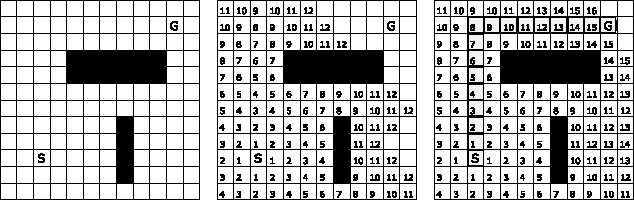
\includegraphics[width=\textwidth]{figs/dijkstragrid.pdf}
    % \def\svgwidth{0.9\textwidth}
    % \import{./figs/}{dijkstragrid.pdf_tex}
    \caption{Dijkstra's algorithm finding a shortest path from `S' to `G' assuming the robot can only travel laterally (not diagonally) with cost one per grid cell. Note the few number of cells that remain unexplored once the shortest path (grey) is found, as Dijkstra would always consider a cell with the lowest path cost first.\label{fig:dijkstragrid}}
\end{figure}

\subsection{A*}\label{sec:astar}\index{A* Shortest Path Algorithm}

Instead of exploring in all directions, knowledge of an approximate direction of exploration to reach the goal may help avoiding the exploration of nodes that are not needed to succeed in the task.
As humans, we can easily interpret the task in \cref{fig:dijkstragrid} and understand that most states in the top-left and bottom-right corner should not be explored if we want to find a solution in a short amount of time.
Such knowledge may be encoded in the search algorithm via a \textsl{heuristic function}\index{Heuristic function}, i.e. an informed guess or estimate of sorts. For example, we could give priority to nodes that have a lower estimated distance to the goal than others.
For this, we would mark every node not only with the actual distance that it took us to get there (as in Dijkstra's algorithm), but also with the estimated cost to target, for example by calculating the Euclidean distance or the \textsl{Manhattan distance}\index{Manhattan distance} between the vertex we are looking at and the goal.
This algorithm is known as A* \cite{hart1968formal}, and illustrated in \cref{fig:astargrid} using the Manhattan distance metric. Depending on the environment, A* might accomplish search much faster than Dijkstra's algorithm, and performs the same in the worst case.

\screencast{https://commons.wikimedia.org/wiki/File:Astar_progress_animation.gif}{astar}

\begin{figure}[htb]
    \centering
    % Note: fonts were not converted to latex here because it was messing around with sizes and everything looked bad.
    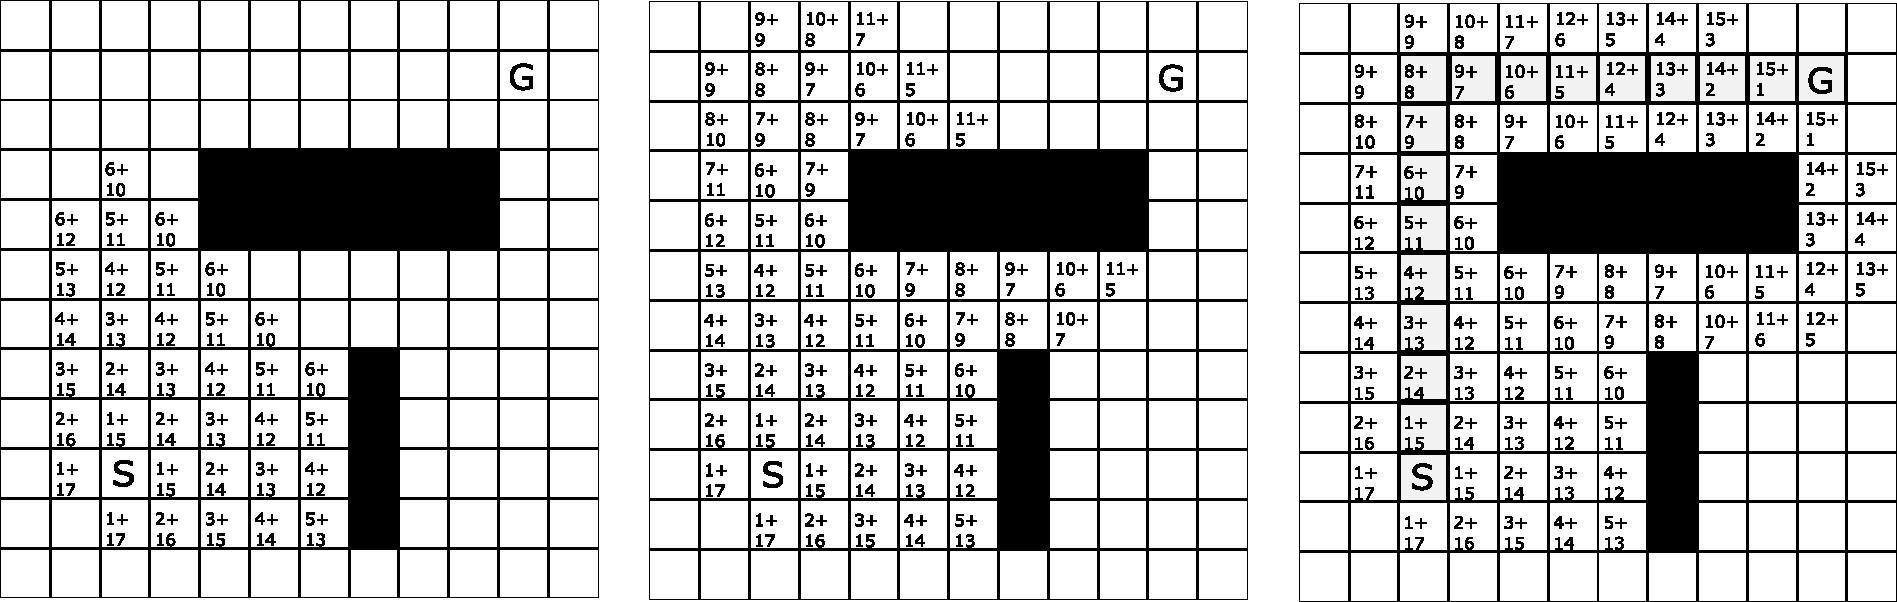
\includegraphics[width=\textwidth]{figs/astargrid.pdf}
    % \def\svgwidth{0.9\textwidth}
    % \import{./figs/}{configurationspace.pdf_tex}
    \caption{Finding a shortest path from `S' to `G' assuming the robot can only travel laterally (not diagonally) with cost one per grid cell using the A* algorithm. Much like Dijkstra, A* evaluates only the cell with the lowest cost, but takes an estimate of the remaining distance into account.\label{fig:astargrid}}
\end{figure}

An extension of A* that addresses the problem of expensive re-planning when obstacles appear in the path of the robot is known as D*\index{D*} \cite{stentz1994optimal}. Unlike A*, D* starts from the goal vertex and has the ability to change the costs of parts of the path that include an obstacle. This allows D* to re-plan around an obstacle while maintaining most of the already calculated path.

A* and D* become computationally expensive when either the search space is large, e.g., due to a fine resolution required for the task, or when the dimensions of the search problem are high (e.g. when planning for an arm with multiple degrees of freedom). Solutions to these problems can be provided by sampling-based path planning algorithms---that are described further below.

\section{Sampling-based Path Planning}

The previous sections have introduced a series of complete algorithms for the path planning problem, algorithms that are guaranteed to (eventually) find a solution if it exists. However, complete algorithms are often infeasible when the possible state space is large, due to practical limitations like available memory or time to execute the algorithm. This is often the case for robots with many degrees of freedom such as arms. In practice, most algorithms are only \textsl{resolution complete}\index{Resolution complete}, meaning they are only complete if the choice of environment resolution is fine enough, as the state-space needs to be somewhat discretized for them to operate and some solutions might be missed as a function of the resolution of the discretization.

Instead of evaluating all possible solutions or using a non-complete Jacobian-based inverse kinematic solution, sampling-based planners create possible paths by using random sampling as the basis for adding points to a tree until some solution is found or time expires. As the probability to find a path approaches one when the number of samples goes to infinity, sampling-based path planners are \textsl{probabilistic complete}\index{Probabilistic complete}. Prominent examples of sampling-based planners are \textsl{Rapidly-exploring Random Trees} (RRT)\index{Rapidly-exploring Random Tree}\index{RRT}\cite{lavalle1998rapidly} and \textsl{Probabilistic Roadmaps}\index{Probabilistic Roadmaps}\index{PRM}(PRM) \cite{kavraki1996probabilistic}. An example execution of RRT for an unknown goal, thereby reducing the continuous path planning problem to a discrete search problem, is shown in \cref{fig:rrt}.

\begin{figure}
    \centering
    \includegraphics[width=\textwidth]{figs/irrt}
    \caption{Counterclockwise from top-left: Random exploration of a 2D search space by randomly sampling points and connecting them to the graph until a feasible path between start and goal is found.\label{fig:rrt}}
\end{figure}

This example illustrates how a sampling-based planner can quickly explore a large portion of space and refine a solution as time goes on. Whereas RRT can be understood as growing a single tree from a robot's starting point until one of its branches hits a goal, probabilistic road-maps create a tree by randomly sampling points in the state-space, testing whether they are collision-free, connecting them with neighboring points using paths that are achievable subject to the kinematics of the robot, and then using classical graph shortest path algorithms to find shortest paths on the resulting structure. The advantage of this approach is that such a probabilistic roadmap has to be created only once (assuming the environment is not changing) and can then be used for multiple queries. PRMs are therefore a \textsl{multi-query} path planning algorithm.\index{Multi-query (path planning)} In contrast, RRTs are known as \textsl{single-query}\index{Single-query (path planning)} path planning algorithms.

In practice, the boundary between the different historic algorithms has become very diffuse, and single-query and multi-query variants of both RRT and PRM exist. It is important to note that there is no `silver bullet' algorithm or heuristic and even their parameter-sets are highly problem-specific. We will therefore limit our discussion on useful heuristics to those that are common to sampling-based planners.

\subsection{Rapidly Exploring Random Trees}
 \screencast{https://youtu.be/Ob3BIJkQJEw}{rrt}
Let $ \mathcal{X}$ be a $ d$-dimensional state-space. It can be helpful to think of this as either the robot's state given in terms of translation and rotations (6 dimensions), a subset thereof, or the joint space with one dimension per joint. Let $ \mathcal{G} \subset \mathcal{X}$ be a  d-ball (d-dimensional sphere) in the state-space that is considered to be the goal, max\_dist the longest permissible edge length, $t$ the allowed time, $k$ the maximum number of vertices to allow in the tree, and goal\_bias the percentage of the time the algorithm should try to connect to a goal state. An RRT planner would proceed as follows:


\begin{verbatim}
Tree=Init(X, G, start, max_dist, t, k, goal_bias);
iteration = 0
WHILE (ElapsedTime() < t AND iteration < k 
AND NoGoalFound(Tree,G)) DO
 iteration = iteration + 1
 IF RandomPercentage() < goal_bias THEN
  q_rand = SampleRandomGoal(G);
 ELSE
  q_rand = SampleRandomState(X);
 ENDIF
 q_nearest = NearestVertex(q_rand)
 q_new = Extend(q_nearest, q_rand, max_dist)
 edge = CreatePath(q_nearest, q_new);
 IF IsAllowablePath(edge) THEN
  Tree.addVertex(q_new);
  Tree.addEdge(edge);
 ENDIF
ENDWHILE
return Tree
\end{verbatim}

This process can be repeated on the resulting tree as long as time allows, and can be implemented with a subset of the input parameters provided above (e.g., without a maximum number of vertices, a maximum timeout duration, or a goal\_bias). RRT is known as an \index{Anytime algorithm} \textsl{Anytime} algorithm, since the algorithm being interrupted will still provide some kind of solution (in this case, a partial graph discretization of the state space). Given a suitable distance metric, the path cost can be stored at each node of the tree, allowing for tracking the shortest path to goal in case there are multiple vertices in the goal region.
%the cost-to-goal can be stored at each node of the tree (much easier if growing the tree from the goal to start), which allows retrieving the shortest path easily. 
There are four key points in this algorithm:

\begin{enumerate}
    \item Finding the next point to add to the tree (SampleRandomGoal, SampleRandomState, and Extend).
    \item Finding out where and how to connect this point to the tree taking into account the robot kinematics (NearestVertex, CreatePath).
    \item Testing whether this path is suitable, i.e., collision-free. (IsAllowablePath)
\end{enumerate}

A prominent method is to pick a random point in the state-space and connect it to the closest existing point in the tree or to the goal, as implemented above. This can require iterating over all nodes in the tree and calculating their distance to the candidate point. Clever selection of data structure for storing the graph can mitigate these costs to be sub-linear in the number of vertices on average. Other approaches put preferences on nodes with fewer out-degrees (those which do not yet have very many connections) and choosing a new point within its vicinity in the direction of the sampled point to add. Both approaches make it likely to quickly explore the entire state-space. Once a new point is sampled, the Extend function uses the max\_dist parameter to limit the maximum edge length, replacing q\_rand with a point on the line connecting q\_nearest and q\_rand that is max\_dist away from q\_nearest.

If there are constraints imposed on the robot's path, for example if the robot needs to hold a cup and therefore is not supposed to rotate its wrist, this dimension can simply be taken out of the state-space.

Once a possible path is found, the space to be sampled from can be reduced to the ellipsoid that bounds the maximal path-length. This ellipsoid can be constructed by mounting a wire of the maximum path length between start and goal and pushing it outward with a pen. Intuitively, only points that are contained by this ellipsoidal area can provide a shorter path than the one currently known, so it is unproductive to attempt to grow the tree elsewhere. This approach is particularly effective when running multiple copies of the same planner in parallel and exchanging the shortest paths once they are found \cite{otte2012}.

\subsection{Connecting Points to the Tree}
A new point is classically connected to the closest point already in the tree or to the goal. This can be done by calculating the distance to all points already in the tree. This does not necessarily generate the shortest path, however. RRT*\index{RRT*} offers a solution to this problem, and is an algorithm that grows the tree in a way that always minimizes the overall path length from the root to every vertex. This is done in two steps: first by connecting new vertices in an optimal way and second by rewiring the tree to make use of this new vertex. By considering all points in the tree within a d-ball (on a 2D map, $d=2$, a circle) from a fixed radius from each added vertex and finding the point that minimizes the overall path length to the start (instead of simply the nearest vertex), we can guarantee that the new vertex is connected on the shortest reachable path from the root of the tree. In the rewiring step, vertices near the newly added vertex are checked to see if an edge from the new vertex to them would result in a shorter path than from their current parent vertex. If this is true, and the edge is allowable (i.e., not in collision or within the physical abilities of the robot), the graph is rewired so the existing vertex is connected with the new vertex as its parent, and it's previous parent edge is removed.

Adding a point to the tree is also a good time to take into account the specific kinematics of a robot, for example a car. Here, a local planner can be used to generate a suitable trajectory that takes into account the orientation of the vehicle at each point in the tree.

\subsection{Collision Checking}
Efficient algorithms for testing collisions deserve a dedicated section. While the problem is intuitive in configuration-space planning in 2D (the robot reduces to a point) and can be solved using a simple point-in-polygon test, the problem is more involved for manipulators that are subject to self-collision.

As collision checking takes up to 90\% of the execution time in the path planning problem, a successful method to increase computational speed is ``lazy collision evaluation''\index{Lazy collision avoidance}. Instead of checking every point for a possible collision, the algorithm first finds a suitable path. Only after does it check every segment of this path for collisions. Segments in collision are deleted and the algorithm continues, but it only keeps the segments of the successful path that were collision-free.

\section{Path Smoothing}
As paths are randomly sampled, they will be most likely shaky and not optimal. For example, a grid-map will generate a series of sharp turns and a sampling-based approach will return zig-zagging paths. Results can be drastically improved by running an additional algorithm that smooths the path. One way of doing this is to connect points of the path using splines, curves, or even trajectory snippets that are known to be feasible for a specific platform. Alternatively, one can also use a model of the actual platform and use a feedback controller such as described in Section~\ref{sec:fbmobile} for mobile robots and Section~\ref{sec:kinematics:inverse:arm} for arms, sample a series of points in front of the robot, and generate a trajectory that the robot can actually drive. When combined with dynamics, this approach is known as \textsl{model-predictive control}\index{Model-predictive control}. Care needs to be taken, however, that the resulting paths are indeed collision free.

\section{Planning at different length-scales}
In practice, no one map representation and planning algorithm might be sufficient. Planning a route for a car, for example, might involve a coarse search over the street network (like one performed by your preferred mapping and navigation app), but not involve planning which lane to actually choose. Planning lanes and how to navigate round-abouts and intersections will necesitate another layer of discrete planning. It may even be preferable to use a sampling-based algorithm to determine how to actually move the robot within a lane and avoid local obstacles. Finally, trajectories need to be turned into wheel speeds and steering angles, possibly using some form of feedback control. This hierarchy is depicted in \cref{fig:planninglayers}. Here, downward-pointing arrays indicate input that one planning layer provides to the one below. Upward-pointing arrows instead indicate exceptions that cannot be handled by the lower levels. For example, a feedback controller cannot handle obstacles well, requiring the sampling-based planning layer to come up with a new trajectory. Should the entire road be blocked, this planner would need to hand-off control the lane-based planner. A similar case can be made for manipulating robots, which also need to combine multiple different representations and controllers to plan and execute trajectories efficiently.

\begin{figure}
    \centering
    % Note: fonts were not converted to latex here because it was messing around with sizes and everything looked bad.
    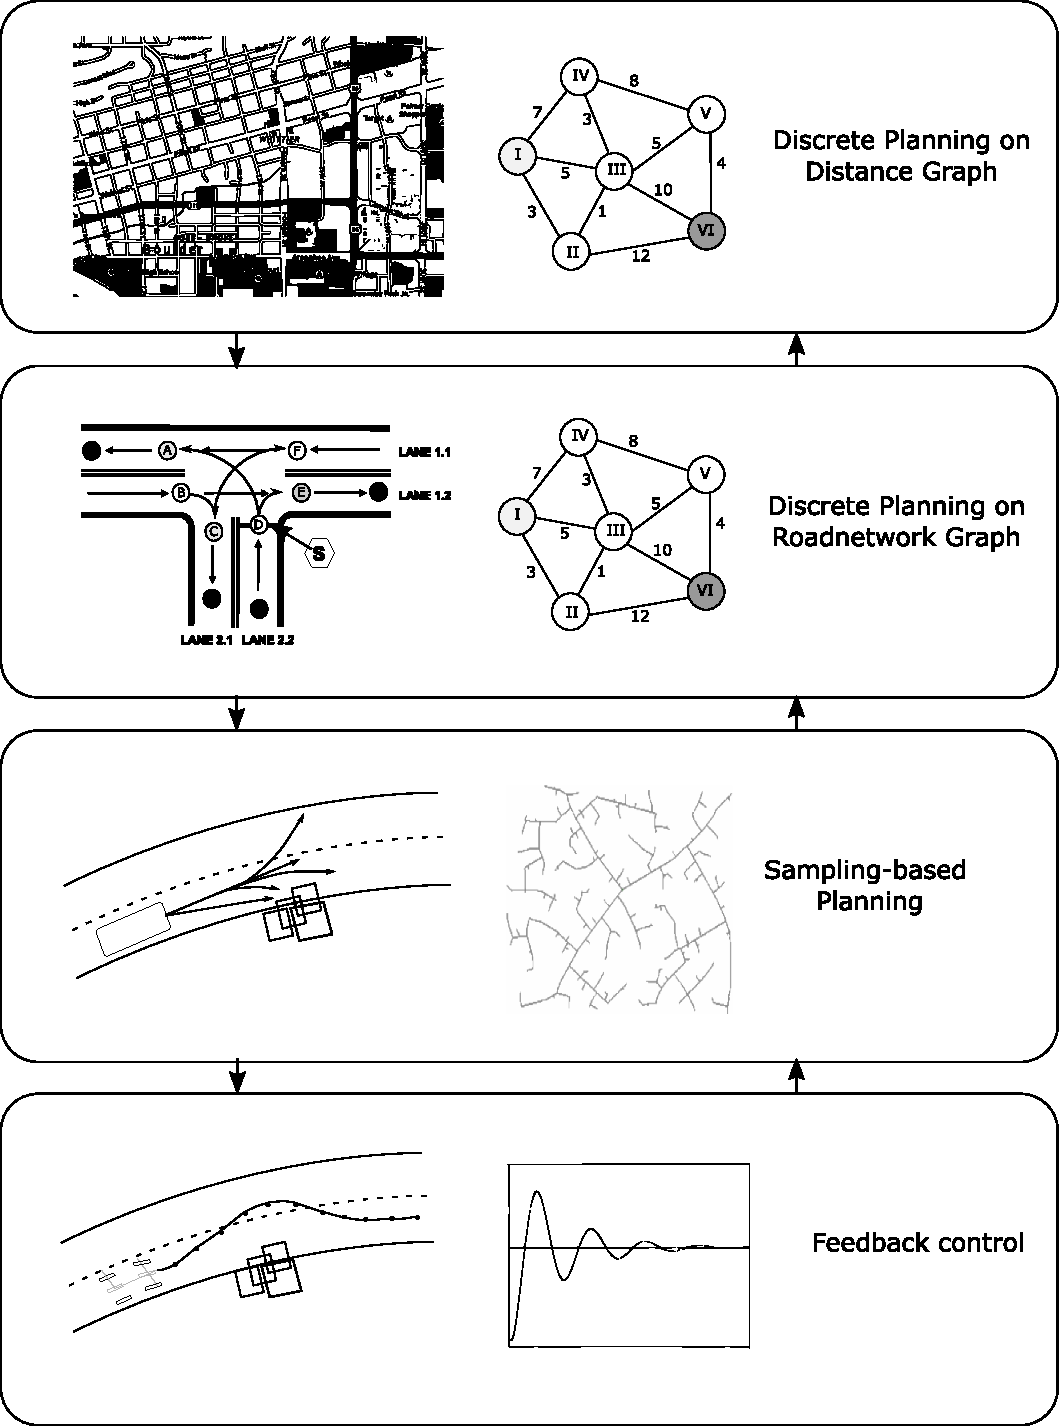
\includegraphics[width=\textwidth]{figs/planninglayers.pdf}
    % \def\svgwidth{0.9\textwidth}
    % \import{./figs/}{planninglayers.pdf_tex}
    \caption{Path planning across different length-scales, requiring a variety of map representations and planning paradigms. Arrows indicate information passed between layers.\label{fig:planninglayers}}
\end{figure}

Note that this representation does not include a reasoning level that encodes traffic rules and common sense. While some of these might be encoded using cost-functions, such as maximizing distance from obstacles or insuring smooth riding, other more complex behaviors such as adapting driving in the presence of cyclists or properties of the ground need to be implemented in an additional vertical layer that has access to all planning layers.


\section{Other path planning applications}

Once the environment has been discretized into a graph, we can employ other algorithms to plan desirable robot trajectories. For example, floor coverage can be achieved by performing a depth-first search (DFS) or a breadth-first-search (BFS) on a graph where each vertex has the size of the coverage tool of the robot. ``Coverage'' is not only interesting for cleaning a floor: the same algorithms can be used to perform an exhaustive search of a configuration space, such as in the example shown in \cref{fig:inversekinematics}, where we plotted the error of a manipulator arm in reaching a desired position over its configuration space. Finding a minimum in this plot using an exhaustive search solves the inverse kinematics problem. Similarly, the same algorithm can be used to systematically follow all links on a website till a desired depth (or actually retrieving the entire world-wide web).

Doing a DFS or a BFS might generate efficient coverage paths, but they are far from optimal as many vertices might be visited twice. A path that connects all vertices in a graph but passes every vertex only once is known as a \textsl{Hamiltonian Path}.\index{Hamiltonian Path} A Hamiltonian path that returns to its starting vertex is known as a Hamiltonian Cycle. This problem is also known as the Traveling Salesman Problem (TSP), in which a route needs to be calculated that visits every city on his tour only once and is known to be NP Complete.\index{Traveling Salesman Problem}


\section{Summary and Outlook}
Path planning is an ongoing research problem. Finding collision free paths for mechanisms with high degrees of freedom such as multiple arms operating in a common space, multi-robot systems, or systems involving dynamics (and therefore adding the derivatives of the state variables to the planning problem) might take unacceptably long to solve.

Although sampling-based path planners can drastically speed up the time to find some solution, they are not optimal and struggle with specific situations such as narrow passages. There is no ``silver bullet'' algorithm for solving all path planning problems and heuristics that lead to massive speed-up in one scenario might be detrimental in others. Also, algorithmic parameters are mostly ad-hoc and correctly tuning them to a specific environment might drastically increase performance.


\section*{Take-home lessons}
\begin{itemize}
\item The first step in path planning is choosing a map representation that is appropriate to the application.
\item The second step is to reduce the robot to a point-mass, which allows planning in the configuration space.
\item This allows the application of generic shortest path finding algorithms, which have applications in a large variety of domains, not limited to robotics.
\item A sampling-based planning algorithm finds paths by sampling random points in the environment. Heuristics are used to maximize the exploration of space and bias the direction of search. This makes these algorithms fast, but neither optimal nor complete.
\item As the resulting paths are random, multiple trials might lead to totally different results.
\item There is no one-size-fits-all algorithm for a path planning algorithm and care must be taken to select the right paradigm (single-query vs.\ multi-query), heuristics, and parameters.
\end{itemize}

\section*{Exercises}\small
\begin{enumerate}
\item How does the computational complexity of Dijkstra's algorithm change when moving from 2D to 3D search spaces?
\item A* uses a ``heuristic'' to bias the search in the expected direction of the goal. Why can it only use a heuristic, not the actual length?
\item Assuming points are sampled uniformly at random in a randomized planning algorithm. Calculate the limiting behaviour of the following ratio (area of points in tree)/(area of points sampled) as the number of points sampled goes to infinity, assuming no duplicates. Assume the total area $A_{total}$ and the area of free space $A_{free}$ within are known.

\item Assuming a kd-tree is used as a nearest-neighbour data structure, and points are sampled uniformly at random, calculate the  run-time of inserting a point into a tree of size $N$. Use ``big-Oh'' notation, e.g. $\mathcal{O}(N)$.

\item What other practical runtime concerns must one consider besides computational complexity alone when doing sampling based motion planning? Can you suggest ways to deal with these other concerns?

\item Write a program that can read in a simple map provided as a textfile where '1' indicate obstacles and '0' indicates free space.
\begin{enumerate}
\item Implement Dijkstra's algorithm to find the shortest path between any two given points in free space.
\item Implement A* to find the shortest path between any two given points.
\item How do these two implementations compare in terms of computational complexity?
\end{enumerate}
\item Write a program that can read an image file in which white areas represent navigable space and black obstacles. Implement a basic RRT algorithm to find the shortest path between any two points.
\item Explore the internet for libraries that implement ``path planning'' in the language of your choice. What tools do you find? How do they define the map? Do they performan obstacle avoidance? Does the kinematics of the robot matter?
\item Extend your path planning implementation for being used with a differential wheel robot. Describe steps that you would need to take for Dijkstra/A* and for RRT.
\item Extend your path planning algorithm for being used with a two-link robot arm. Would you plan in joint or in configuration space, and what are advantages and drawbacks of each?
\item How does the computational complexity change when moving from a single 6-DoF robot arm to a torso with two 6-DoF robots? Can you think about an approach that maintains the original computational complexity? What are the drawbacks of this approach.
\item Consider a robotic assembly task in which a robot retrieves objects from a known location and assembles them on a table. When can you rely on simple inverse kinematics and when do you need path planning?
\item How does a planning problem change when you not only consider positions, but also forces and torques? Could you use  a variation of RRT to solve such a problem?
\item Download a robotic path planning tool that allows you to try different algorithms.
\begin{enumerate}
\item Compare solution quality and speed among the different solutions.
\item What do you need to take into account when using randomized planners? Is comparing single-shot experiments sufficient?
\end{enumerate}
\end{enumerate}

\normalsize
